\documentclass[10pt]{extarticle}
\usepackage[utf8]{inputenc}
\usepackage{cite}
\usepackage{graphicx}
\graphicspath{ {./images/} }
\usepackage{wrapfig}

\title{M33's Future Density Profile and Star Formation Rate}
\author{Samantha Andrews}
\date{March 2020}

\begin{document}

\maketitle

\section{Introduction}
Andromeda and our own Milky Way are on a collision course. However, these two galaxies will not be the only ones whose physical properties will change due to the collision. M33, a late type spiral in our Local Group \cite{2018ApJ...864...34S}, will also be changed forever once this collision occurs. The major question is how. How will the internal structure of M33 be changed, and how will its evolution be effected? 

Semczuk et al have studied the possibility of a past interaction between M33 and M31 where they got to within 37  kpc of each other. Observations point to the two being gravitationally bound to each other. Simulations give strong evidence that the two galaxies did interact in the past hinted at by the bridge like structure between the two \cite{10.1111/j.1745-3933.2008.00528.x}. It has been proposed that the interaction occurred 4-8 Gyr ago, and is the reason M33 has a warped HI region. This gaseous warp is thought to be due to the tidal forces and ram pressure from M31 \cite{2018ApJ...864...34S}. Lokas et al has done simulations for tidal stirring of disk galaxies orbiting a Milky Way like host \cite{_okas_2015}. It is believed that this leads to dwarf spheroidal galaxies, and is dependent on a resonance between the angular velocity
of the stars in the dwarf and its orbital motion. Because of this resonance, tidal stirring has occurred. 

Another reason it is believed M31 and M33 collided is because they both experienced a burst in their star formation rates (SFR). Bernard et al. has studied through simulations that when two galaxies have a close encounter, a burst in SFR occurs \cite{10.1111/j.1365-2966.2011.20234.x}. When the interaction is believed to have occurred, the SFR of M33 was approximately three times larger than its normal rate, putting it at $0.6 \times 10^{-9} M_{\odot} yr^{-1} pc^{-2} $.

\section{The Proposal}
In this project I will address the following questions:
\subsection{Questions}
\begin{enumerate}
  \item What is the stellar disk density profile as a function of time?
  \item What profile fits and does it change? Is it a sersic profile?
  \item Is there evidence for tidal truncation?
  \item What can we infer about the SFR from the density profile? Will there be a burst in star formation?
\end{enumerate}

\subsection{Approach}
From the data we have the time, particle type, mass of the particle, position and momentum. Using this information, we were able to create a mass breakdown for M33 in a previous homework. In another homework, we were able to compute the mass profile for each galaxy in our local group, and fit it with a profile. By using that mass profile, I will be able to create a density profile. I can then attempt to fit it with a Sersic Profile given by \begin{equation}
    I(r) = I_e e^{-7.67((r/R_e)^{1/n}-1}
\end{equation}
which is in terms of the effective radius, or, the half light radius. In Lab 6, we assumed a mass to light ratio of one for the stellar bulge. Therefore, the luminosity is proportional to the stellar mass, which we can find in the mass breakdown of M33. By solving for $I_e$ in \begin{equation}
    L = 7.2I_e \pi R_e^2
\end{equation}

we can plug it into Equation 1, and therefore have the Sersic Profile we can use an array of radii to find the best fit. I will \begin{wrapfigure}{l}{0.5\textwidth}
    \centering
    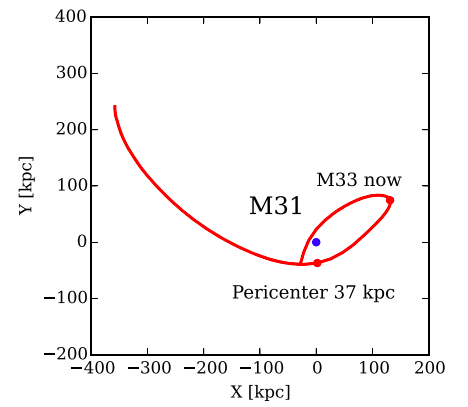
\includegraphics[width=0.5\textwidth]{Orbit.png}
    \caption{M33's orbit done by Semczuk et al}
    \label{fig:orbit}
\end{wrapfigure}plot the density profile with its corresponding Sersic profile. From the density profile, we can infer the gas density and thus what will happen to the star formation rate as M31 and the MW collide. It would also be interesting to create a graph similar to one given by Semczuk et al in Figure \ref{fig:orbit}

for the expected orbit of M33 when M31 and the Milky Way collide. This would not only show M33's expected orbit, but also tell how close M33 would get to the collision, and see if it would eventually also collide which a previous homework alluded to. 


\subsection{Hypothesis}
My hypothesis is that there will be an increase in the SFR because I expect the density profile will increase with time. We have discussed that as galaxies get close together, we can expect there to be a star formation burst. I also expect there to be tidal truncation since M33 is tidally locked and close to M31, and we determined its orbit will decay and possibly also collide. 

\bibliographystyle{plain}
\bibliography{references}


\end{document}
